\part{Infrastrucuture as a Service -- IaaS}

%%%%%%%%%%%%%%%%%%%%%%%%%%%%%%%%%%%%%%%%%%%%%%%%%%%%%%%%%%%%%%%%%%%%%%%%%%%
\begin{frame}
\frametitle{IaaS -- Components}
\begin{columns}
\column{.3\textwidth}
\begin{itemize}
\item Images
\item Instances
\item Block storage
\item Object storage
\item Network
\end{itemize}
\column{.7\textwidth}
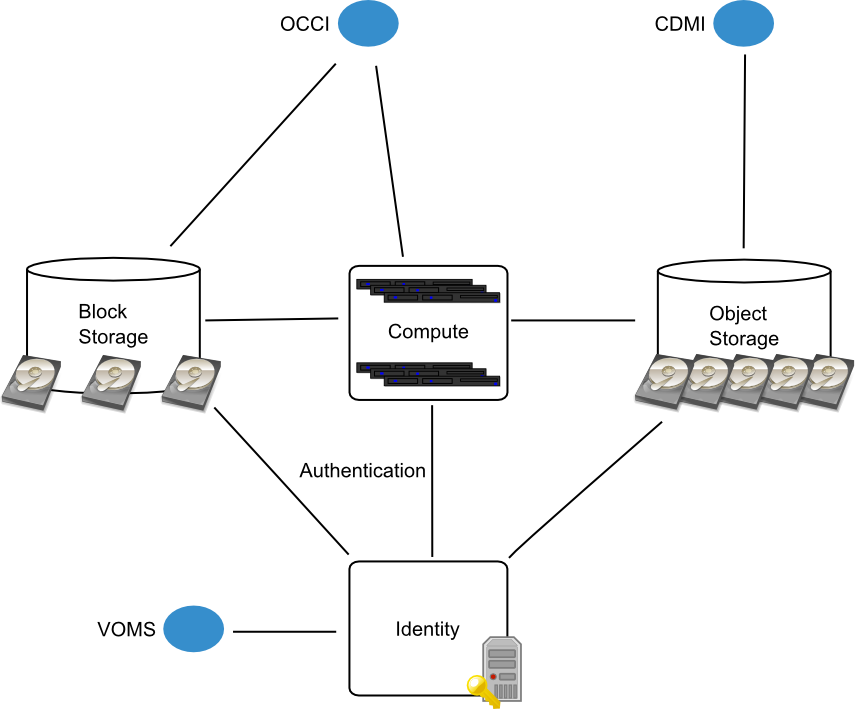
\includegraphics[width=\textwidth]{images/IaaS_OCCI.png}
\end{columns}
\end{frame}

%%%%%%%%%%%%%%%%%%%%%%%%%%%%%%%%%%%%%%%%%%%%%%%%%%%%%%%%%%%%%%%%%%%%%%%%%%%
\begin{frame}
\frametitle{IaaS -- What is an image?}
\framesubtitle{}
There are various answers to this question
\begin{itemize}
\item Typically
  \begin{itemize}
  \item A blob of data representing the contents of a disk or file system
  \item Usually contains the root file system contents of an operating system
  \end{itemize}
\item Application data can be conveyed within images
\item Image is usually used as a term for a \emph{template} to create
  a virtual machine or \emph{instance} of it.
%% another wonderful diagram showing the relations among image and instance
%% will add additional relations later on, e.g. block storage volumes
\end{itemize}
\end{frame}

%%%%%%%%%%%%%%%%%%%%%%%%%%%%%%%%%%%%%%%%%%%%%%%%%%%%%%%%%%%%%%%%%%%%%%%%%%%
\begin{frame}
\frametitle{IaaS -- What is an instance?}
\framesubtitle{}
\begin{itemize}
\item A virtual machine (VM)
  \begin{itemize}
  \item ... created from an \emph{image}
  \item ... given an amount of \emph{resources}
  \item ... and additional parameters (aka. \emph{user-data})
  \end{itemize}
\end{itemize}
\end{frame}

%%% Local Variables:
%%% TeX-master: "2014-05-23_Best_Practices"
%%% End:
